\documentclass{bioinfo}
\copyrightyear{2016} \pubyear{2016}

\access{Advance Access Publication Date: Day Month Year}
\appnotes{Original Paper}

\begin{document}
\firstpage{1}

\subtitle{Systems Biology}

\title[One model to rule them all]{One model to rule them all}
\author[Steiert \textit{et~al}.]{Bernhard Steiert\,$^{\text{\sfb 1,}*}$, Jens Timmer\,$^{\text{\sfb 1,2}}$ and Clemens Kreutz\,$^{\text{\sfb 1}}$}
\address{$^{\text{\sf 1}}$Institute of Physics, University of Freiburg, Germany and \\
$^{\text{\sf 2}}$BIOSS Centre for Biological Signalling Studies, University of Freiburg, Germany.}

\corresp{$^\ast$To whom correspondence should be addressed.}

\history{Received on XXXXX; revised on XXXXX; accepted on XXXXX}

\editor{Associate Editor: XXXXXXX}

\abstract{\textbf{Motivation:}
A major goal in systems biology is to reveal potential drug targets for cancer therapy.
Signaling pathways triggering cell-fate decisions are often altered in cancer resulting in uncontrolled proliferation and tumor growth.
However, addressing cancer-specific alterations experimentally by investigating each node in the signaling network one after the other is difficult or even not possible at all.\\
\textbf{Results:} Here, we combined quantitative time-resolved data from different cell lines with non-linear modeling under L1 regularization, which is capable of detecting cell-type specific parameters.
To adapt the least-squares numerical optimization routine to L1 regularization, sub-gradient strategies as well as truncation of proposed optimization steps were implemented.
Likelihood-ratio test is used to determine the optimal penalization strength resulting in a sparse solution in terms of a minimal number of cell-type specific parameters that is in agreement with the data.
The uniqueness of the solution was investigated using the profile likelihood.
Based on the minimal set of cell-type specific parameters experiments were designed for improving identifiability and to validate the model.
The approach constitutes a general method to infer an overarching model with a minimum number of individual parameters for the particular models.\\
\textbf{Availability:} The algorithm is implemented within the freely available, open-source modelling environment Data2Dynamics \cite{Raue2015} based on MATLAB. Source code for all examples is provided online at ...\\
\textbf{Contact:} \href{bernhard.steiert@fdm.uni-freiburg.de}{bernhard.steiert@fdm.uni-freiburg.de}\\
\textbf{Supplementary information:} Supplementary data are available at \textit{Bioinformatics}
online.}

\maketitle

\section{Introduction}
The progress in the development of experimental assays like the establishment of high-throughput measurement techniques raised new demands on statistical methodology. 
Many scientific questions in the field of Bioinformatics and Systems Biology nowadays requires large models with hundreds or even thousands of parameters or variables. 
Therefore, a major issue in many applications is feature selection, i.e. determination of informative parameters or variables which are required to explain experimental observations, for identification of differential expression and/or for making reliable predictions. 

In many cases, feature selection is equivalent to model discrimination \citep{Box67} since a set of features corresponds to a specific model with corresponding set of parameters. 
In \emph{multiple linear regression}, as an example, feature selection corresponds to choosing appropriate prediction variables used to fit an experimentally observed response variable. 
The traditional approach for choosing a suitable level of detail and the respective optimal set of features is iteratively testing many models \citep{Thompson1978}, 
i.e.~different combinations of features e.g.~by \emph{forward-} or \emph{backward selection} or combinations thereof \citep{Hocking1967, Efroymson60}. 
However, if the number of potential predictors is are large, the number of possible combinations increase dramatically rendering such iterative procedures as infeasible. 

Regularization techniques have been suggested as an alternative approach for selecting features and estimating the parameters in a single step. 
The idea is to estimate the parameters by optimization of an appropriate objective function, e.g.~by maximizing the \emph{likelihood}. 
If then in addition the impact of individual features is penalized, the optimal solution becomes sparse and the level of sparsity can be controlled by the strength of penalization. 
It has been shown that such penalties are equivalent to utilization of prior knowledge supplemental to the information provided by the data. 

The additional information provided by penalties reduce the variance of the estimated parameters but at the same time introduce a bias. This effect has been termed as \emph{shrinkage}. 
If the regularizing penalties are chosen appropriately, e.g. if the \emph{L0}- or \emph{L1-norm} are applied, a second effect occurs which can be utilized for feature selection. 
Because the L0- and L1-norm penalize parameters unequal to zero, only parameters remain in the model which are mandatory for explaining the data. 
Since the penalized likelihood is discontinuous for L0 regularization, L1-penalties are usually preferred.

The concept of using the L1-norm for data analysis and calibrating a model has been applied in several fields like for deconvolution of wavelets \citep{Taylor1979}, 
reconstruction of sparse spike trains of Fourir components \citep{Levy1981}, recovering acoustic impedance of seismograms \citep{Oldenburg1983} 
as well as for \emph{compressed sensing} \citep{Candes2008,Cheng2015} and clinical prediction models \citep{Hothorn2006}. 
Additionally, it has been used to establish statistical methods which are robust against violation of distributional assumptions about measurement errors \citep{Claerbout73, Barrodale1973}. Moreover, L1 penalties have been applied to incorporate \emph{Laplacian priors} \citep{xx}. 
%
Despite this variety of applications, the usability for feature selection and a comprehensive statistical interpretation was not established until introduction of the 
\emph{LASSO (least absolute shrinkage and selection operator)}. 
This prominent approach for linear models was published in \cite{Tibshirani94} when the first cheap high-throughput techniques were available and the necessity of new approaches for analyzing high-throughput data became inevitable.

The standard LASSO has been generalized or adapted for other applications in several directions. 
Feature selection via LASSO was discussed for the regression case in more detail in \cite{tibshirani96}, for Cox-regression in \cite{Tibshirani1997}, and for clustering e.g.~in \cite{Witten2010}
The \emph{elastic net} has been introduced as a combination of L1 and L2 regularization \citep{Zou05}. 
The so-called  \emph{group-LASSO} has been established to select between predefined groups of features \citep{Yuan2006}, \emph{fused LASSO} accounts for additional constraints of pairs of parameters \citep{Tibshirani2005}, and  \emph{generalized LASSO} has been developed to regularize arbitrary prespecified parameter linear combinations \citep{Tibshirani2011}.


Mechanistic  \emph{ordinary differential equation (ODE)} models are applied in Systems Biology for describing and understanding cellular signal transduction pathways or gene regulatory networks. 
For such ODE models, the feature selection issue occurs, if several cell types are considered. 
Since each cell type has different concentrations of intracellular compounds and diverse structure, each parameter of a reaction network could potentially be different. 
We suggest L1-regularization in this setting to predict parameters which differ between cell-types.
The components of mechanistic models have counterparts in the biological pathway of interest. 
Therefore, the models usually contain a large number of state variables representing molecular compounds and many parameters for the individual biochemical interactions. 
Therefore, the models are large and the effect of the parameters on the dynamics is typically strongly nonlinear. 
For estimating parameters in such ODE models, only a small subset of optimization routines in combination with appropriate strategies for calculating derivatives of the objective function, dealing with non-identifiability, handling of local minima etc. are applicable \citep{Raue2013}. 
We therefore augment an existing and well-tested implementation for parameter estimation for such systems \citep{Raue2015} to perform feature selection based on L1-regularization. 
For this purpose, trust-region optimization \citep{Coleman96} was combined with a subgradient strategy as presented in \citep{Schmidt09} to enable efficient optimization in the presence of L1-penalties. 

Since shrinkage, i.e. decreasing the variance by introducing a bias is not intended for mechanistic models, we only select the features, i.e. the cell-type specific parameters, by L1-regularization and then use these additional features to estimate the magnitude of the parameters in an unbiased manner. 
A suitable strategy is presented for choosing the regularization strength in this setting. 
The applicability is demonstrated using a benchmark model from the \emph{DREAM (Dialogue for Reverse Engineering Assessment and Methods)} parameter estimation challenge \citep{Steiert12}. 
The presented approach constitutes a suitable methodology for predicting cell-type specific parameters as well as for identification of cell-type specific sensitivities for drugs which are prominent issues in cancer research.

\section{Problem statement}

Given a model $\mathcal M$ describing the kinetics of reaction network components $x_i$ with $i \in [1,\dots,m]$ by a system of ordinary differential equations (ODE)
\begin{equation}
\dot x(t) = f(x(t),u(t,p_u),p_x)\label{eq:ode}
\end{equation}
with solutions $x(t)$ representing concentrations of molecular compounds, for external inputes $u(t)$.
States $x$ are mapped to experimental data $y$ using an observation function $g$, yielding
\begin{equation}
y(t) = g(x(t),p_y)+\epsilon(t,\sigma) \:.\label{eq:obs}
\end{equation}
The error $\epsilon \sim \mathcal N(0,\sigma)$ is assumed to be normally distributed in the following.
Initial concentrations $p_0$, as well as parameters $p_x$ of the ODE, $p_u$ of the input, $p_y$ of the observation function, $\sigma$ of the error model, are subsumed in the parameter vector
\begin{equation}
p = [p_0, p_x, p_u, p_y, \sigma] \:.\label{eq:par}
\end{equation}
Therefore, the expressions (Eq~\ref{eq:ode}-\ref{eq:par}) fully specify $\mathcal M$.
To ensure positive values and improve numerics, all parameters are log-transformed.\\
Now given two cell types whose data can be fitted by a common ODE structure (Eq.~\ref{eq:ode}) but the results differ in their parameters $p$, i.e. $p_1 \neq p_2$.
Discovering which of the components in $p_1$ and $p_2$ are cell type-specific is the main topic of this manuscript.

\begin{figure}[!tpb]%figure1
\centerline{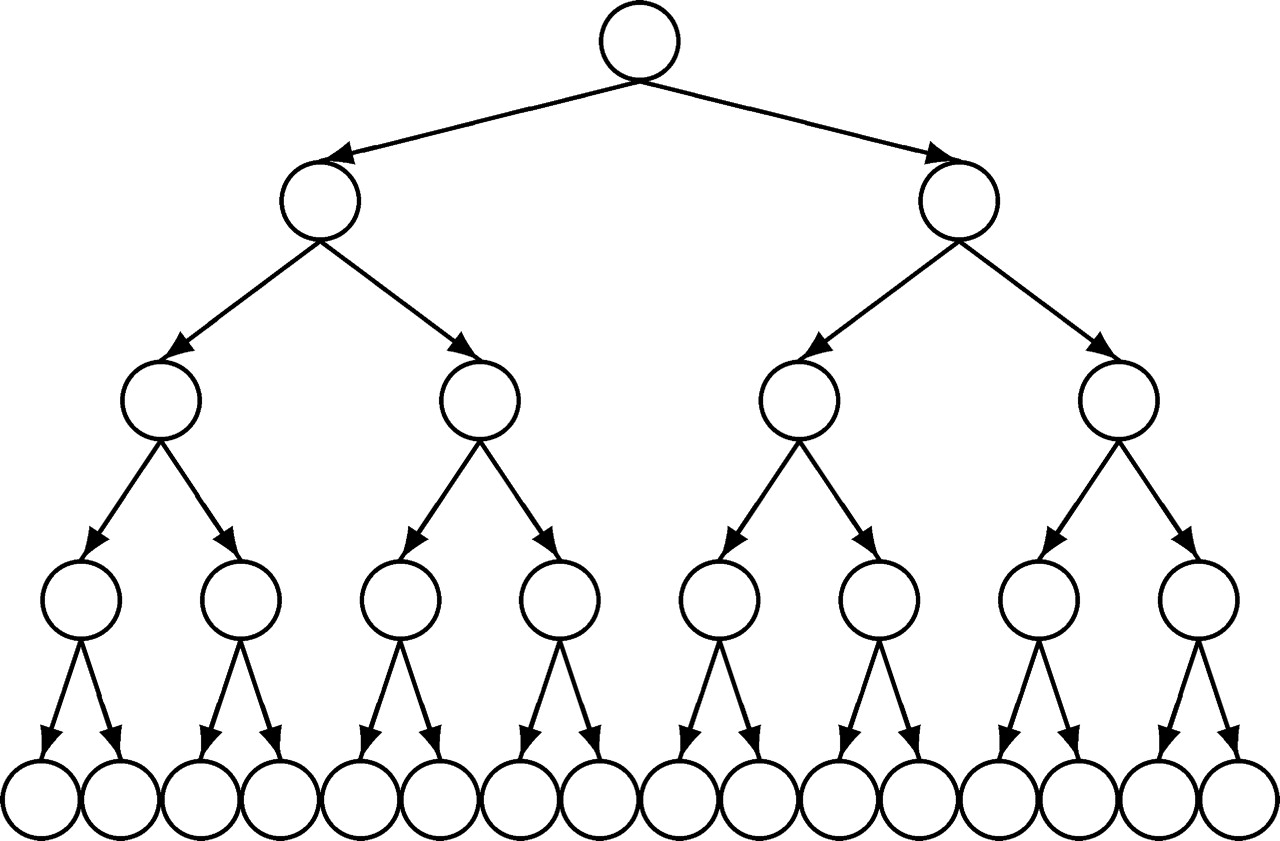
\includegraphics[width=235pt]{Figures/tree.jpg}}
\caption{Naive approach.}\label{fig:01}
\end{figure}

\subsection{Unbiased parameter estimation}

To estimate parameters $p$ for $n$ data points ${y_i}$, given values of the correspoding observation function observation $g(t_i,p)$, the negative two-fold log likelihood
\begin{equation}
-2\log \mathcal L(p) = \sum_{i=1}^n \frac{(y_i-g(t_i,p))^2}{\sigma_i^2} =: \chi^2\label{eq:lik}
\end{equation}
is optimized, resulting in the maximum likelihood estimate
\begin{equation}
\hat p = \text{arg}\min \left[ -2\log \mathcal L(p) \right] \:.
\end{equation}
Multi-start deterministic local optimization is applied to ensure that $\hat p$ is in fact the global optimum.

\subsection{Regularization}
Regularization is often applied to incorporate prior knowledge or to improve numerics of parameter estimation.
Here, we persue a different strategy.
Regularization is used to assess the fold-change $\tilde r_i = 10^{r_i}$ of parameters between two cell types, i.e. $p_1 = \tilde r \cdot p_2$.
Thus, a posterior
\begin{equation}
-2\log \mathcal L_{L_k}(p,r) = -2\log \mathcal L(p) + \lambda \sum_i ||\log \tilde r_i||_k\label{eq:likreg}%\vspace*{-4pt}
\end{equation}
is implemented consisting of the likelihood (Eq.~\ref{eq:lik}) and a $L_k$ regularization term, weighted by $\lambda$.
The regularization term corresponds to a prior in a Bayesian framework:
For $k=0$ the $L_0$ prior is a delta distribution, for $k=1$ the $L_1$ prior is Laplacian function, and for $k=2$ the $L_2$ prior is a Gaussian function.\\
Different metrics $L_k$ show different properties.
$L_0$ would be ideal for our task due to its' direct penalization of the number of $r_i \neq 0$.
However, $L_0$ is not recommended because the associated optimization problem is known to be NP-hard.
In general, for $k<1$, the $L_k$ metric is non-convex which severly hampers parameter estimation.
On the other hand, both $L_0$ and $L_1$ induce sparsity and under some conditions they even give the same results on selection.
In contrast, $L_k$ for $k>1$ does not give sparse results, $L_2$ for instance is efficient but not sparse.
In that sense, the $L_1$ metric is unique, because it is the only one which combines both features, convexity and sparsity.
Therefore, we use $k=1$ in the following.\\
Due to local optima, the MLE (Eq.~\ref{eq:lik}) is obtained for individual cell types.

\begin{figure}[!tpb]%figure1
\centerline{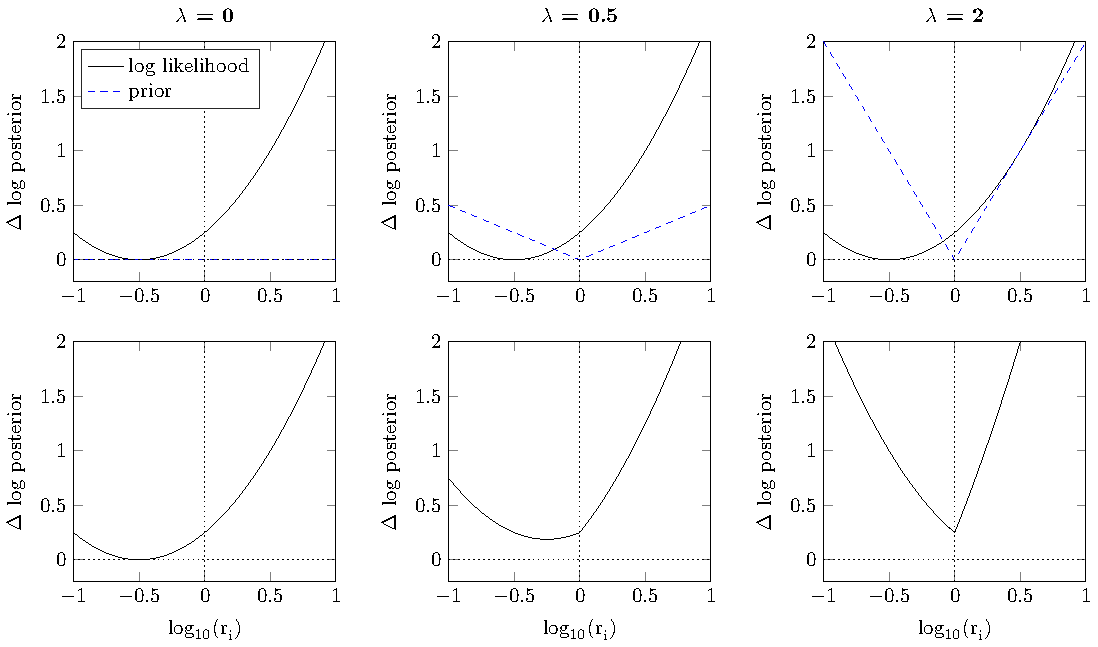
\includegraphics[width=235pt]{Figures/l1_cartoon_priorstrength.pdf}}
\caption{Posterior for different $\lambda$.}\label{fig:01}
\end{figure}

\subsection{Regularized parameter estimation}
Optimization in context of partially observed stiff non-linear coupled ODE is non-trivial.
However, methods have been developed to efficiently solve this problem.
To augment the existing implementations with $L_1$ regularization, i.e. to minimize
\begin{equation}
	-2\log \mathcal L_{L_1}(p,r) = -2\log \mathcal L(p) + \lambda \sum_i |r_i|
\end{equation}
the following considerations are necessary.
Efficient optimization routines often exploit the quadratic form in (Eq.~\ref{eq:lik}).
For example, the implementation of a trust-region method \textit{lsqnonlin} in Matlab expects residuals
\begin{equation}
	\text{res}_i = \frac{y_i-g(t_i,p)}{\sigma_i}
\end{equation}
as input and implicitely converts these to a likelihood.
To implement optimization of the posterior (Eq.~\ref{eq:likreg}),
\begin{equation}
	\text{res}_i = \sqrt{\frac{|r_i|}{1/\lambda}}
\end{equation}
is appended to the residuals vector.
The associated sensitivites are given by
\begin{equation}
	\text{sres}_i = \frac{\text{sgn}(r_i)}{\frac{2}{\lambda}\sqrt{\frac{|r_i|}{1/\lambda}}} \:.\label{eq:sres}
\end{equation}
Therefore, the gradient
\begin{equation}
	g = 2 \: \text{res}_i \cdot \text{sres}_i = \pm \lambda
\end{equation}
matches the theoretical value.
For $\lambda = 0$, Eq.~\ref{eq:sres} is not defined.
The convergence criterion is given by
\begin{equation}
	\begin{cases}
	\nabla_i \chi^2(\hat r_i) + \lambda \text{ sign}(\hat r_i) = 0, \:\:& |\hat r_i| > 0\\
	|\nabla_i \chi^2(\hat r_i)| \le \lambda, \:\:&\hat r_i = 0 \:.
	\end{cases}
\end{equation}
To incorporate this criterion into optimization, $\text{sres}_i$ is set to $0$ if $|\nabla_i \chi^2(\hat r_i)| \le \lambda$.\\
% sub-gradient

\subsection{Profile likelihood}

Used to check results (parameter should not be compatible with 0)\\
Used to check uniqueness: Test model with 1 additional parameter in comparison to parsimonious model.
If inside CI, a parameter that was different to 0 is now compatible with 0, one cannot decide on the data which one is different.

\begin{figure}[!tpb]%figure1
\centerline{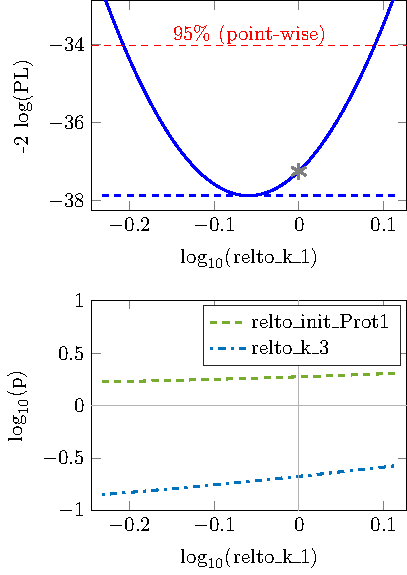
\includegraphics[width=110pt]{Figures/relto_k_1.pdf}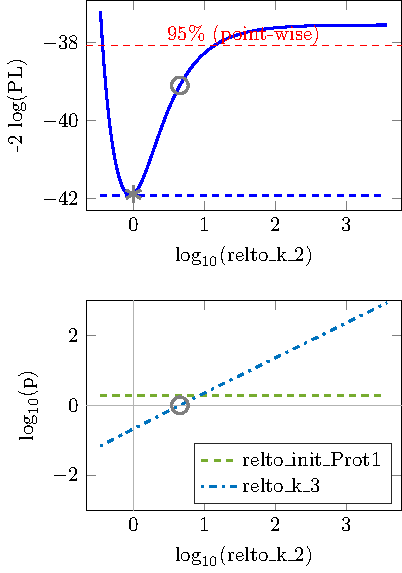
\includegraphics[width=110pt]{Figures/relto_k_2.pdf}}
\caption{Uniqueness and exchangeability.}\label{fig:01}
\end{figure}

\subsection{Regularization strength $\lambda$}
Increase $\lambda$ until mismatch between model and data is large enough to reject simplification.\\
Several methods: Cross-Val, LRT, AIC, BIC \\ \\

\begin{figure}[!tpb]%figure1
\fboxsep=0pt\colorbox{gray}{\begin{minipage}[t]{235pt} \vbox to 100pt{\vfill\hbox to
235pt{\hfill\fontsize{24pt}{24pt}\selectfont FPO\hfill}\vfill}
\end{minipage}}
%\centerline{\includegraphics{fig01.eps}}
\caption{Regularization path. Show different selection criteria (LRT, AIC, BIC).}\label{fig:01}
\end{figure}

%Equation~(\ref{eq:01}) Text Text Text Text Text Text  Text Text
%Text Text Text Text Text Text Text Text Text Text Text Text Text.
%Figure~2\vphantom{\ref{fig:02}} shows that the above method  Text
%Text Text Text  Text Text Text Text Text Text  Text Text.
%\citealp{Boffelli03} might want to know about text text text text
%.....


\begin{methods}
\section{Approach}
Given an overarching model that is able to describe two cell types with parameter vectors $p_1$ and $p_2$ for cell types 1 and 2, respectively.
Eq.~\ref{eq:likreg} is used to $L_1$ penalize the fold-change parameters $r$.
Then, $\lambda$ is scanned and the number of cell type specific parameters is observed.
For chosing the optimal $\lambda$, the un-regularized Eq.~\ref{eq:lik} is optimized, under the constraint that parameters with $r_i = 0$ are shared between both cell types.\\
Uniqueness, Validation design (= find dynamics with a small prediction CI, which are different for ct1 and ct2)\\ \\
%
%Text Text Text Text Text Text  Text Text Text Text Text Text Text
%Text Text Text Text Text Text Text Text.
%Figure~2\vphantom{\ref{fig:02}} shows that the above method  Text
%Text Text Text Text Text Text Text Text Text  Text Text.
%\citealp{Boffelli03} might want to know about text text text
%text\vspace*{1pt}
%
%\begin{itemize}
%\item for bulleted list, use itemize
%\item for bulleted list, use itemize
%\item for bulleted list, use itemize\vspace*{1pt}
%\end{itemize}
%
%Text Text Text Text Text Text  Text Text Text Text Text Text Text
%Text Text Text Text Text Text Text Text.
%Figure~2\vphantom{\ref{fig:02}} shows that the above method Text
%Text Text Text Text Text Text Text Text Text Text Text.
%\citealp{Boffelli03} might want to know about text text text text
%Text Text Text Text Text Text  Text Text Text Text Text Text Text
%Text Text Text Text Text Text Text Text.
%
%Text Text Text Text Text Text  Text Text Text Text Text Text Text
%Text Text  Text Text Text Text Text Text\vadjust{\newpage}.
%Figure~2\vphantom{\ref{fig:02}} shows that the above method  Text
%Text Text Text  Text Text Text Text Text Text  Text Text.
%\citealp{Boffelli03} might want to know about text text text text
%
%
%\subsection{This is subheading}
%
%Text Text Text Text Text Text Text Text Text Text Text Text Text
%Text Text  Text Text Text Text Text Text.
%Figure~2\vphantom{\ref{fig:02}} shows that the above method  Text
%Text Text Text Text Text Text Text Text Text  Text Text.
%\citealp{Boffelli03} might want to know about  text text text text
%Text Text Text Text Text Text  Text Text Text Text Text Text Text
%Text Text  Text Text Text Text Text Text.
%
%
%\subsubsection{This is subsubheading}
%
%Text Text Text  Text Text Text Text Text Text  Text Text.
%\citealp{Boffelli03} might want to know about  text text text text
%Text Text Text Text Text Text Text Text Text Text Text Text Text
%Text Text  Text Text Text Text Text Text.
%Figure~2\vphantom{\ref{fig:02}} shows that the above method  Text
%Text Text Text  Text Text Text Text Text Text  Text Text.
%\citealp{Boffelli03} might want to know about  text text text text
%
%\enlargethispage{6pt}
%
%
%Text Text Text Text Text Text  Text Text Text Text Text Text Text
%Text Text  Text Text Text Text Text Text.
%Figure~2\vphantom{\ref{fig:02}} shows that the above method  Text
%Text Text Text  Text Text Text Text Text Text  Text Text.
%\citealp{Boffelli03} might want to know about  text text text text


\end{methods}

\begin{figure}[!tpb]%figure1
\centerline{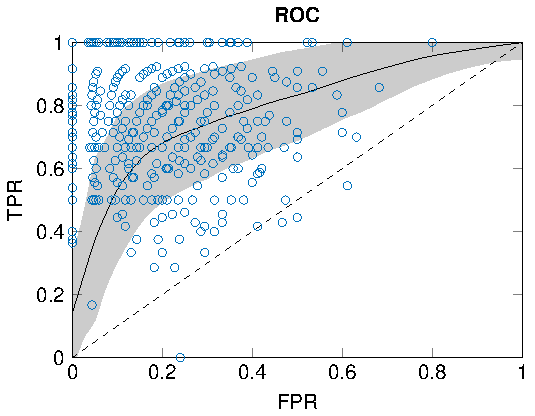
\includegraphics[width=235pt]{Figures/ROC.pdf}}
\caption{DREAM6 results. No experimental design. $N = 150$. Black line is average ROC curve. Shading is standard deviation. Blue circles denote selected model for all iterations. Because the dots appear on average near the maximum of sensitivity and specificity (upper left corner), the selection criterion is appropriate.}\label{fig:01}
\end{figure}

%\begin{figure}[!tpb]%figure2
%%\centerline{\includegraphics{fig02.eps}}
%\caption{Caption, caption.}\label{fig:02}
%\end{figure}

%Text Text Text Text Text Text  Text Text Text Text Text Text Text
%Text Text  Text Text Text Text Text Text.
%Figure~2\vphantom{\ref{fig:02}} shows that the above method  Text
%Text Text Text  Text Text Text Text Text Text  Text Text.
%\citealp{Boffelli03} might want to know about  text text text text\vspace{10pt}

\section{Application}
DREAM6 Model 1\\
Gene-regulatory network\\
Used to evaluate performance of experimental design strategies to optimize parameters and predictions\\ \\
Description model:\\
6 state mRNA, 6 states Protein\\
Initials fixed\\
29 parameters\\
1 p\_degradation\_rate\\
6 pro\_strength\\
6 rbs\_strength\\
8 $K_d$\\
8 Hill\\
Use gold-standard as cell type 1\\
All parameters identifiable (except 1 Hill only lb)\\
1/3 of parameters is assumed to be cell type-specific / were changed in cell type 2\\
Randomly simulated fold-changes of [2 5 10] for non-Hill and [2 4] for Hill; and inverse; Hill such that they stay inside [1 4]\\ \\
Description data:\\
mRNA measurements with 21 data-points, all observed\\
Protein measurements with 41 data-points, 2 observed\\
Observation function is identity\\
Error model is absolute + relative with given parameters\\
Wildtype all observed\\
3 possible perturbations per node: Knock-out, knock-down, over-expression\\
In total, budget was sufficient for around 9 additional data-sets\\
Strategy: Choose random (50\%) if perturbation is selected\\
Choose random if mRNA (1/3) or proteins (2/3) are observed, if so choose random 2 proteins\\ \\
Approach:\\
Use $L_1$ and scan along $\lambda$ for variable selection\\
Use unpenalized solution for selection of $\lambda$\\
Iterate 1000 times\\ \\
Results:\\
ROC curve\\
Performance for different parameter types\\
Performance for different fold-changes

\begin{table}[!t]
\processtable{Performance of algorithm on DREAM6 M1\label{Tab:01}} {\begin{tabular}{@{}llll@{}}\toprule Parameter class &
nTested & Sensitivity & Specificity\\\midrule
Protein degradation rate & row1 & row1 & row1\\
Protein production strength & row2 & row2 & row2\\
Ribosomal strength & row3 & row3 & row3\\
$K_d$ value & row3 & row3 & row3\\
Hill coefficient & row4 & row4 & row4\\\botrule
\end{tabular}}{Calculations took xx.xx min on an Intel Xeon E5-1620 3.60Ghz workstation.}
\end{table}


%Text Text Text Text Text Text  Text Text Text Text Text Text Text
%Text Text  Text Text Text Text Text Text.
%Figure~2\vphantom{\ref{fig:02}} shows that the above method  Text
%Text Text Text  Text Text Text Text Text Text  Text Text.
%\citealp{Boffelli03} might want to know about  text text text text
%
%
%Table~\ref{Tab:01} shows that Text Text Text Text Text  Text Text
%Text Text Text Text. Figure~2\vphantom{\ref{fig:02}} shows that
%the above method Text Text. Text Text Text  Text Text Text Text
%Text Text. Figure~2\vphantom{\ref{fig:02}} shows that the above
%method Text Text. Text Text Text  Text Text Text Text Text Text.
%Figure~2\vphantom{\ref{fig:02}} shows that the above method Text
%Text.









%%%%%%%%%%%%%%%%%%%%%%%%%%%%%%%%%%%%%%%%%%%%%%%%%%%%%%%%%%%%%%%%%%%%%%%%%%%%%%%%%%%%%
%
%     please remove the " % " symbol from \centerline{\includegraphics{fig01.eps}}
%     as it may ignore the figures.
%
%%%%%%%%%%%%%%%%%%%%%%%%%%%%%%%%%%%%%%%%%%%%%%%%%%%%%%%%%%%%%%%%%%%%%%%%%%%%%%%%%%%%%%






\section{Discussion}

Differences to linear setting.\\
Parameters are not necessarily monotoneous.\\
Scanning $\lambda$ not necessarily globaly optimal.\\
Regularization might induce additional local optima that could be globally optimal.\\
Numerics tough in the vicinity of 0.\\
\begin{equation}
	H_{ij} \approx \text{sres}_i \cdot \text{sres}_j = \frac{\text{sgn}(r_i)}{\frac{2}{\lambda}\sqrt{\frac{|r_i|}{1/\lambda}}} \cdot \frac{\text{sgn}(r_j)}{\frac{2}{\lambda}\sqrt{\frac{|r_j|}{1/\lambda}}}
\end{equation}
\begin{equation}
	\lim_{r_i \rightarrow 0} H_{ij} = \lim_{r_j \rightarrow 0} H_{ij} = \pm \infty
\end{equation}
L1.x does not help either (not sparse)\\
Combos do not help either (in vicinity of 0, $L_1$ diminates anyway.\\
Check cross-validation\\
Check shrinkage\\
L2 might be an option --> Daniel\\ \\
DREAM specific discussion\\
Lack of observation function\\
No differences in initials\\
Hills hard to detect (range is important)\\
Experimental design principles were not applied\\
Method data driven

%(Table~\ref{Tab:01}) Text Text Text Text Text Text  Text Text Text
%Text Text Text Text Text Text  Text Text Text Text Text Text.
%Figure~2\vphantom{\ref{fig:02}} shows that the above method  Text
%Text Text Text  Text Text Text Text Text Text  Text Text.
%\citealp{Boffelli03} might want to know about  text text text text
%
%\begin{enumerate}
%\item this is item, use enumerate
%\item this is item, use enumerate
%\item this is item, use enumerate
%\end{enumerate}
%
%Text Text Text Text Text Text Text Text Text Text Text Text Text
%Text Text Text Text Text Text Text Text.
%Figure~2\vphantom{\ref{fig:02}} shows\vadjust{\pagebreak} that the
%above method  Text Text Text Text Text Text Text Text Text Text
%
%
%Text Text Text Text Text Text  Text Text Text Text Text Text Text
%Text Text  Text Text Text Text Text Text.
%Figure~2\vphantom{\ref{fig:02}} shows that the above method  Text
%Text Text Text\vspace*{-10pt}


\section*{Acknowledgements}

Text Text Text Text Text Text  Text Text.  \citealp{Boffelli03} might want to know about  text
text text text\vspace*{-12pt}

\section*{Funding}

This work has been supported by the... Text Text  Text Text.\vspace*{-12pt}

\bibliographystyle{natbib}
%\bibliographystyle{achemnat}
%\bibliographystyle{plainnat}
%\bibliographystyle{abbrv}
% \bibliographystyle{bioinformatics}

% \bibliographystyle{plain}

\bibliography{document}

\end{document}
